\documentclass[11pt]{book}
\usepackage{geometry}        
\geometry{letterpaper}    
\usepackage[parfill]{parskip}  
\usepackage{graphicx}
\usepackage{amssymb}
\usepackage{epstopdf}
\usepackage{tabularx}
\usepackage{minitoc}
\usepackage{pdfpages}
\DeclareGraphicsRule{.tif}{png}{.png}{`convert #1 `dirname #1`/`basename #1 .tif`.png}

\usepackage[colorlinks=true, pdfstartview=FitV, linkcolor=blue, 
            citecolor=blue, urlcolor=blue]{hyperref}


\newtheorem{theorem}{Theorem}
\newtheorem{corollary}[theorem]{Corollary}
\newtheorem{definition}{Definition}
\newtheorem{lemma}{Lemma}
\newtheorem{exercise}{Exercise}
\newtheorem{remark}{Remark}
\newtheorem{example}{Example}
\newtheorem{warning}{Warning}

\def\grad{ \mbox{grad}}
\def\curl{ \mbox{curl}}
\def\div{ \mbox{div}}
\def\U{\ensuremath {\cal U}}
\def\S{\ensuremath {\cal S}}
\def\V{\ensuremath {\cal V}}
\def\R{\ensuremath {\cal R}}
\def\tr{\ensuremath {\mbox{tr}}}




% ------------------- Title and Author -----------------------------
\title{Project Report\\
TDT4290 - Customer Driven Project \\ "Privacy Advisor"}
\author{GROUP 4\\Ulf Nore, Nicholas Gerstle, Henrik Knutsen, Dimitry
  Kongevold,\\ Einar Afiouni, Neshahvan Karunakaran, Amanpreet Kaur}
\date{NTNU, Fall 2011}
\begin{document}


\frontmatter
\maketitle

\chapter*{\centering Abstract}
This is report for the "Privacy Advisor" project in the TDT4290 - Customer Driven
Project course. The "Privacy Advisor"
software was developed as part of a larger project for SINTEF ICT, in
order to investigate the applicability of machine learning to aid users in
making internet privacy decisions. Previous research at SINTEF has pointed
out several advantages to using a Case Based Reasoning (CBR) agent as
a core algorithm in this type of application, which this project implements. SINTEF ICT
has indicated the use of the project software as part of future
research and therefore the emphasis was placed on implementing a broad
framework, rather than actual algorithms.

The resulting product is a Java based framework with a central CBR
engine that is extensionable with respect to key algorithms, databases
and user interfaces. It also allows for network communication with a
community server that could implement a collaborative filtering approach 
similar to the CBR.

%more details in results?

\dominitoc

\listoftables
\listoffigures
\tableofcontents

\pagenumbering{arabic}


\chapter{Introduction}

This report describes the development of a machine learning systems for aiding users in Internet privacy decisions. The software is titled "Privacy Advisor" and uses a case based reasoning (CBR) approach, which is a learning method that seeks to predict preferences based on previous user choices. The project is a part of the course TDT4290 - Customer Driven Project and is a part of a SINTEF ICT research project in privacy agents. The report is written in a chronological order where each chapter represents a distinct "phase" in the development process. In reality, of course, there are no crisp boundaries, but the structure here provides a useful structure for reasoning about the process. 

The structure of the report is as follows. Part~\ref{p1} describes the initial phase of the project; the projects directive (Chapter~\ref{directive}), the planning phase (Chapter~\ref{plan}) and the preliminary study phase (Chapter~\ref{prelim}). The project directive gives a high level overview over the project, its objectives, how they are reached, project scope, resources available etc. The preliminary study comprise the first weeks of the project, and is a consistent effort to better grasp the problem at hand, identify how it can be broken into subproblems and what tools are required to solve these problems. It also seeks to identify to some extent what the priorities in the project are; that is, given scarce resources, which objectives are prioritized. The project planning phase seeks to make a more fine grained decision on how resources are best allocated over time and to the various tasks that comprise the project.

Part~\ref{p2} describes the requirements specification (Chapter~\ref{reqspec}), design phase, implementation and documentation. The requirements specification is a contract between the customer and the project team where the the requirements to be satisfied by the software are stated explicitly. Based on the requirements, a design (Chapter~\ref{design}) is made, which is to serve as a guideline for implementing (Chapter~\ref{impl}) the software system.

Finally, Part~\ref{p3} describes the testing and evaluation phase, and summarizes the project.

\part{Initial Phase - Planning and Research}\label{p1}
\addtocounter{chapter}{1}
\setcounter{section}{0}
% Activate the following line by filling in the right side. If for example the name of the root file is Main.tex, write
% "...root = Main.tex" if the chapter file is in the same directory, and "...root = ../Main.tex" if the chapter is in a subdirectory.
 
%!TEX root =  

\chapter{Project Directive}
This document describes the mandate, background, resources available and organizational structure of the project �A Privacy Advisor�, henceforth referred to as �the project�.

\section{Mandate}
The purpose of this project is to implement the key functionality of a privacy agent as described in Nyre and T�ndel (2010), that provides users with advice in making Internet privacy decision. 


\subsection{Background}
This project is a part of a larger research project at SINTEF ICT that studies approaches to handling Internet privacy related issues. The underlying idea is that while users are often concerned about the way various websites and services handle private information about them, obtaining information about this is very costly as privacy policies tend to be very long documents formulated in an inaccessible language. This has led to the idea that Internet privacy can be handled by machine learning techniques, where a particular decision is based on the user�s past behavior and the behavior of similar users.

Nyre and T�ndel has then proposed a �Privacy Agent� structure that uses the case based reasoning (CBR) method for giving privacy advice. CBR is in many ways similar to the way human experts reason about problems, and is usually described as a process in four stages (here related to the privacy decision problem):
\begin{itemize}
\item Retrieve: 
Given a new site, the agent will retrieve from its knowledge base, the set of cases deemed the most similar to the one at hand. This means, that if presented with the site Facebook, for instance, the agent finds Twitter, Google and LinkedIn to be the sites that have the most similar policy to Facebook.
\item Reuse: 
Look at the decisions made about the cases that were found and adapt this decision to the problem at hand. In this case, the agent needs to see if there are strong enough indications toward a particular behavior with respect to the type of site that is at hand. If for instance, the user has accepted the policies of all the similar sites found, he is also likely to accept that of Facebook.
\item Revise: 
Once a conclusion is reached, it is presented to the user (along with the background for why it is reached). The user may then choose to accept the conclusion, or to overrule it, providing the system with directions as to why it was wrong. This may in turn cause the agent to update its parameters accordingly. 
\item Retain: Finally, the new case is stored to the database along with the user�s decision as a reference for the next time the same site is opened, and as a case to employ when evaluating new sites.
\end{itemize}

Nyre and T�ndel also describes this local CBR approach to be complemented by a community database where the same information is stored, allowing for a second lookup that uses a collaborative filtering, that is, making a decision based on the behavior of similar users.

\section{Objectives}
This project identifies three key objective, arranged by order of importance:
Implementing a testing framework of CBR based privacy agent that is able to make privacy decisions based on previous user behavior.
Implement the community system/collaborative filtering part of the agent.
Extend the system to other standards for machine readable privacy policies.
Implement the system as a browser plugin. This is considered least important, and is contingent on the success of early testing. It is also given a low priority given the relative small portion of major websites that implement P3P.


\section{Resources and Duration}
The system in its complete form is to be demonstrated on November 24 2011. For the project period, a total of 25 hours per week per project member is planned. With seven group members and a project spanning 13 weeks, this adds up to approximately 2300 hours.

\section{Organization}
The project group organization is based on the modules of the system that is being implemented. One group member is responsible for developing one particular feature. This organization is shown in Table~\ref{orgTable}.

\begin{table}[htdp]
\caption{Responsibilities}
\begin{center}
\begin{tabularx}{\textwidth}{| X | X | X |}
\hline
\textbf{Role} & \textbf{Description} &\textbf{Responsible} \\
\hline
Administrative 	&  Customer relations  & Ulf Nore \\
			& Requirement specification & \\
			& Requirement specification & \\
			& Planning documents & \\
			& Meeting minutiae & \\
			& Project report & \\	
\hline					
Software design and Architecture   	&  UML modeling.	 	& Nicholas Gerstle \\ 
						      	& Design report.		& \\
							& User documentation.	& \\
							& Technical Decisions.	& \\
\hline
Data Storage/Databases	& Flat file data storage system. 	& Amanpreet Kaur \\
					& Database systems	.			& \\
\hline
CBR - Algorithms and Data structures 	& Data structures for storing privacy policy information.	& Dimitry Kongevold,\\
								& Define and implement similarity metrics.			& Neshahavan Karunakaran \\
								& Retrieval and learning algorithms. &	\\
								& Parameter storage. & \\
\hline
Testing and Evaluation 	& Design test cases. & Henrik Knutsen \\
					& Criteria/methodology for model testing. & \\
\hline
GUI & Implement a simple GUI for testing model framework. & Ulf Nore \\
\hline
Version control & Set up and maintain code repository. & Einar Afiouni \\
\hline
XML/P3P Parser & Implement P3P parser that produces inputs to CBR & Einar Afiouni \\
\hline
Version control & Set up and maintain code repository. & Einar Afiouni \\								 	
\hline
\end{tabularx}
\end{center}
\label{orgTable}
\end{table}%



\section{Planning}
A project plan has been developed for the purpose of communicating expectations and progress within the group and to the customer and the advisor. The plan also serves as an aid in identifying problems and project management. For the software development process, a hybrid waterfall model has been chosen.


\section{Limitations and Scope}
The primary focus of this project is on developing a framework that allows for testing the CBR privacy agent framework. This entails building a module for parsing policy documents in XML format, a data structure for holding policy information in memory (henceforth �policy objects�), a set of exchangeable distance metric that compares policy objects, a generic retrieval algorithm (such as k Nearest Neighbors) that works with any distance metric and methods to store and update a knowledge base. Being a part of an ongoing research project, reusability and modularity are important success factors for in evaluating the project. This means that it should for instance be simple to swap P3P with some other privacy policy standard, that different distance metrics should be applicable, new metrics could easily be implemented and so forth.


\setcounter{section}{0}
\addtocounter{chapter}{1}
% Activate the following line by filling in the right side. If for example the name of the root file is Main.tex, write
% "...root = Main.tex" if the chapter file is in the same directory, and "...root = ../Main.tex" if the chapter is in a subdirectory.
 
%!TEX root =  

\chapter{Preliminary Study\label{prelim}}


\minitoc

This section describes the preliminary study phase of the project. It focuses on gaining insight into the problem the software system is to solve. For this project, the problem is very well defined from the customer's perspective as such, little time is spent looking into similar products and various possible solutions to the overarching problem of computer aided privacy advice.

A large portion of this time was spent on investigating the proposed solution and the technologies involved, that is Case Based Reasoning (CBR) and the technologies used by it. As the customer, SINTEF ICT, is a research institution, and the project can somewhat simplified be viewed as the "implementation" part of a larger research project, the customer could from the start provide relatively clear specification of the system that is envisioned\footnote{The system is outlined in broad terms in the article Inger Anne T{\o}ndel, {\AA}smund Ahlmann Nyre and Karin Bernsmed: \emph{"Learning Privacy Preferences"}, SINTEF ICT 2011.}. 

Another critical work laid down in this phase were choices with respect to project scope and development model. As will become apparent, these choices are strongly related to the nature of the problem statement.

\section{Internet Privacy Technology}

This section briefly describes the situation today with respect to the sate of Internet privacy, current Internet privacy tools and which needs the project seeks to address.

\subsection{What is Internet Privacy?}
Privacy is the means or ability of an individual to seclude himself or information about himself from third parties and selectively controlling what personal information\footnote{The term \emph{personal information} will here refer to information such as name postal and e-mail address, financial information, social security number and so forth.}it  about him is to be available. When talking about \emph{Internet privacy}, it is referred to the control over the type and amount of private information that is revealed under a transmission of data over the Internet, and hereunder, who has access to the information. The legal framework setting the boundaries of the service providers' priveliges with private information is very marginal, and typically, the best information available for users is through the provider's \emph{privacy policy}.

The article "User Agents for Matching Privacy Policies with User Preferences"\footnote{Karin Bernsmed, {\AA}smund Ahlmann Nyre and Martin Gilje Jaatun: "User Agents for Matching Privacy Policies with User Preferences", SINTEF ICT.} describes the rationale for a system aiding users in making Internet privacy decisions in terms of a \emph{privacy paradox} - the fact that while most users claim to put great emphasis on privacy, this is not mirrored in their actions.

Social networks such as Facebook provide a good illustration of this paradox and why it is important. Such services have grown to major prominence as a means of communication over the last half decade, and a common trait of these networks is the sharing of more private information than what was common on the "traditional'' Internet. This is all well and fine, as long as the information is shared in the appropriate sphere, but there are obviously issues once your private images or derogatory comments appear in the public sphere, something that has been related through several news stories. 


\subsection{Current Privacy Technology}\label{privTech}
The disproportion between the average Internet user's concern for privacy and the actual control he has over private information referred to as the privacy paradox above, as well as the very fact that privacy is a \emph{fundamental human right} is obviously something that calls for action. While most websites provide a privacy policy, these tend to very long documents written in a obscure "legalesque" language, intended  for protecting the websites' interests than those of users. To aid users in understanding the implications of such policies and hence in making informed privacy related decisions, there is a need for tools providing users with information about policies in a format that is accessible to the user. As pointed out in the abovementioned paper, current technologies are often hard to configure and requires domain knowledge from the user or may be more concerned with hiding information\footnote{Ie. \emph{anonymity}. While this certainly aids in protecting privacy, it also renders certain services such as social networks useless, since a sharing a certain level of private information is required for the service to have any meaning. As an example of this approach, see instance the Tor Project: https://www.torproject.org/.}, rather than the consequences of sharing information which is a common activity in online shopping and social networks.

\subsubsection{The Platform for Privacy Preferences Project (P3P}
As an aid in this problem, machine readable standards such as P3P have been introduced. P3P seeks to compress the information contained in the privacy policy in an XML document that can be parsed and summarized by computer programs. 

The AT\&T \emph{Privacy Bird} is mentioned in T{\o}ndel et al. (2011) as an example of current P3P based Internet privacy software. Privacy Bird can parse P3P documents and match a site's privacy policy with the user's preferences. The problem with this however, is that the user has to explicitly state his preferences, which, first of all, is a rather time-consuming endeavor. Secondly, while a user may have clear notions about which information he would share in a \emph{particular} situation, such preferences may be very hard to generalize. It may be hard to give a general statement on privacy preferences in a way that is both simple enough for the user to understand and rich enough to actually describe the problem. Furthermore, preferences may be inconsistent, for instance, while in the general case, the user would not accept privacy terms similar to those of for instance Facebook; however in Facebook's particular case he will accept them nevertheless.

\subsection{How Machine Learning Can Improve Privacy Advice}
The novel feature of this project is to introduce an intelligent system that \emph{learns} the user's preferences, seeking to limit the amount of user interference. This is to be achieved by the use of CBR agent, that can look at previous examples of user choices in similar situations. A particular advantage of the CBR approach is the feedback loop where the system can actually \emph{explain} its choice in terms of similar cases which sets CBR apart from alternative reasoning models such as artificial neural networks. It also allows for better tuning to user response in those cases that the user disagrees with the recommendation.

\section{Case Based Reasoning}
Being, the core part of the system to be developed, some time needed to be spent on looking into CBR. In vague terms, CBR is problem solving based on past solutions to previous problems. This approach is similar in many ways to the way humans solve problems, both as domain experts, and in their daily life. For instance, a software engineer, faced with a particular problem, may identify similarities to a problem he has previously solved, using for instance a factory design pattern, so he adopts this solution to the new problem with some modifications. Similarly, a NTNU student, hungry for a late night snack, recalling past experience with favorable opening hours and culinary excellency, heads off to Sesam.

\begin{figure}[htbp]
\begin{center}
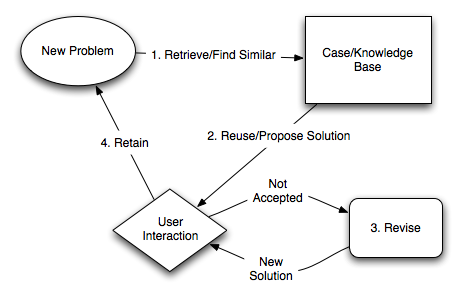
\includegraphics[width = .75\textwidth]{PrelimStudy/cbr}
\caption{A Simplified CBR Cycle.}
\label{cbrCycle}
\end{center}
\end{figure}


For computer implementation, CBR is usually formalized in terms of a four step process:

\begin{itemize}
\item Retrieve: 
Given a new site, the agent will retrieve from its knowledge base, the set of cases deemed the most similar to the one at hand. This means, that if presented with the site Facebook, for instance, the agent finds Twitter, Google and LinkedIn to be the sites that have the most similar policy to Facebook.
\item Reuse: 
Look at the decisions made about the cases that were found and adapt this decision to the problem at hand. In this case, the agent needs to see if there are strong enough indications toward a particular behavior with respect to the type of site that is at hand. If for instance, the user has accepted the policies of all the similar sites found, he is also likely to accept that of Facebook.
\item Revise: 
Once a conclusion is reached, it is presented to the user (along with the background for why it is reached). The user may then choose to accept the conclusion, or to overrule it, providing the system with directions as to why it was wrong. This may in turn cause the agent to update its parameters accordingly. 
\item Retain: Finally, the new case is stored to the database along with the user�s decision as a reference for the next time the same site is opened, and as a case to employ when evaluating new sites.
\end{itemize}

As can be seen from this specification, CBR is a very generic approach, and several notions need to be defined before it can be implemented. For instance, we need to settle on a knowledge representation. For most CBR purposes, a frame based approach is taken. To store this knowledge representation, an appropriate database structure must be selected, and a routine for keeping this up to date must be established. Given a representation, one needs to define a notion of \emph{similarity} between cases, and an algorithm to do the actual retrieval. Usually, one would also like this algorithm to provide some measure of the certainty of the results as well.

While SINTEF has proposed some initial ideas for how these details can be implemented, they are very much open problems, and subject to empirical study to find an 'optimal' approach for the actual problem at hand.

\section{Project Scope}
The research nature of this project makes it a very open-ended one. The clearly most important part of the system envisioned by the customer is the CBR engine, that classifies websites based on the user's previous decisions. Implementing this is clearly necessary, regardless of which direction is followed and what limitations are made.

However, once the local CBR engine and auxiliary modules such as parsing P3P documents and so forth are in place, there are several directions that the project can take, and pursuing all of them is an unlikely scenario given the resource limitations. To some extent, the direction of the project also depends in a large extent on how well preliminary testing goes; that is, how well does the CBR system actually predict user preferences. Depending on the results of these tests, several possible directions were deemed possible:

\begin{enumerate}
\item Given test failure, making improvements to the algorithm, hereunder, the retrieval methods, the amount of data stored per case, the distance metric used to compare cases, and the weighting of the different features of a case/policy.
\item Extending the system by implementing the community portion/collaborative filtering part of the proposed system.
\item Given a test success, implementing a working browser plugin.
\item Closely related to the previous point, extending the system to work with other privacy policy standards.
\end{enumerate}

Direction 1 above takes the project from a system engineering direction more over to a scientific and statistical analysis type project, and while placing some emphasis on tuning the algorithms, this is not our primary focus\footnote{This would require gathering a dataset of some size as well as setting up testing scenarios, which not only requires a sophisticated statistics background, but also likely group of test users. It was decided that this should not be prioritized in a software engineering project of limited scope such as this.}. Item 3 relies heavily on the effectiveness of the algorithm and may require exactly the type of statistical analysis discussed. In agreement with the customer, it was therefore concluded that the collaborative filtering part was to be the second focus after the CBR part. 

\section{Development Model and Workflow}
Having briefly identified and outlined the project "flow", a development method or model must be chosen. A two-stage implementation process is envisioned; the first in which the core CBR is implemented. In the second part, the focus is on the community/CF portion. By thus splitting the work in two stages, time is made available for more thorough testing and reworking of the CBR portion, while work on the CF system, which is given a lower priority is pushed back. Given this project flow, we deemed that the work fits well within waterfall model framework. This is described in more detail in the next section. 


\subsection{The Waterfall Model}
The waterfall model describes the development process as a linear process that starts with planning and requirements specification, and flows sequentially through design, implementation and finally (in this case) testing as is illustrated in Figure~\ref{waterfall}. Arguments \emph{for} the waterfall approach is that it encourages rigorous planning and design, which means that inconsistencies and problems can be discovered earlier in the process, which is generally less costly than if they are discovered late, since this often means re-writing a large portion of code. 

Another advantage of the waterfall model, which relates directly to the nature of this particular project, is the focus on design. Since the software product to be delivered is a very early prototype that is to be used in further research, and likely to be further modified in the future, providing solid modularity and interfaces so as to allow code reuse is critical. Properly documenting the program structure, as encouraged by the waterfall model, will also be highly beneficial to anyone who is later to modify the program.

\begin{figure}[htbp]
\begin{center}
\includegraphics[width = 1.0\textwidth]{PrelimStudy/workflow}
\caption{The Waterfall Model.}
\label{workflow}
\end{center}
\end{figure}

A common criticism raised against the waterflow model is that development rarely occurs in completely distinct stages; it is often hard to completely finish one phase of the project before moving on to the next. For instance, in many projects, requirements may be subject to uncertainty or change, so that design in turn must be altered. While recognizing this and other inherit weaknesses in the waterflow model, we think that for this project, requirements are quite clear, and since its scope is limited, a slightly modified waterfall model will still serve the project well. 

Among the modifications that we have made is, as indicated in Figure~\ref{workflow}, a slight overlap between the different phases. This is justified by the fact that some stages are not dependent entirely on the previous stage. For instance, given a detailed design, a test plan and testing procedures can be worked out independently, and testing of one module does not require the entire system to be integrated.

\setcounter{section}{0}
\addtocounter{chapter}{1}
% Activate the following line by filling in the right side. If for example the name of the root file is Main.tex, write
% "...root = Main.tex" if the chapter file is in the same directory, and "...root = ../Main.tex" if the chapter is in a subdirectory.
 
%!TEX root =  

\chapter{Planning Phase}
\label{plan}

\minitoc 

\subsection*{Purpose}
This chapter details the planning process that seeks to identify the different phases in the development process and allocate resources over time to the various activities that comprise each phase. Planning also needs to account for a number of risk factors that may impact the process, either by allowing for enough preventive measures or by allocating extra time to activities that may be affected. Thus a risk report enumerating several potential risks has been worked out.

\section{Project Phases}\label{phases}
The choice of development model is detailed in Chapter \ref{prelim}. Here the various phases of the project are described.

\subsection{Preliminary Study and Research}
In this phase the aim is for each project member to acquire a certain level domain knowledge in the field of Internet privacy and to learn the necessary technology and tools required to implement the model as proposed by the customer. This entails having a working knowledge of the Java programming language, version control using Git and the CBR framework.

\subsection{Planning}
Planning seeks to identify the activities needed to reach the project objective. This entails breaking down the objectives into sub-problems, identifying the relationship between these, and allocating time for each of them. 

\subsection{Requirement Specification}
The requirements specification is a document listing the functional and non-functional requirements of the software to be developed, which is a standard that the results is to be measured against, thus serving as not only a contract between the customer and the project team, but as a basis for developing testing methods.

\subsection{Design/Architecture}
This phase consists of a broad structuring and specification of the overall system. It defines the program structure in terms of program flow, modules, classes and interfaces as well as coding standards and other conventions that will serve as guidelines for the implementation phase.

\subsection{Implementation}
In this phase the design is realized as a working Java program according to the models developed in the Design phase. 

\subsection{Evaluation and Documentation}
This phase consists of testing the system and documenting the structure of the system and how it is operated. From a software engineering perspective, the primary testing grounds are against the standards prescribed by the requirements specification rather than applicability of the applicability of the CBR agent model to privacy enhancement. As mentioned, among the primary objectives of the project is to provide a testing framework to verify the applicability of the given system in making privacy decisions.

\subsection{Ongoing Activities}

\subsubsection{Reporting and Administrative Tasks}
Under this heading are more project management related activities, such as routine organizational work (ie. arranging meetings and writing status updates), more refined distribution of tasks as the project is underway, and preparation of the project report (this document).

\subsubsection{Study and Lectures}
To solve several of the problems posed by this project, most group members have had to learn new tools and technologies. This includes, but is not limited to Case Based Reasoning, version control (Git), certain features of Java and so on. Lectures on project management  and software development are also subsumed under this heading.

\section{Risk Report}\label{riskReport}
The term \emph{risk} is usually defined as the possibility of an undesirable outcome (loss) as a consequence of a choice or an action made. 


\subsection{Overview and Risk Management}
In this section some risk factors that can impact the project are indentified. Every project does risk management at some level, wether explicit stated or not. By identifying and quantifying the \emph{likelihood} and \emph{consequence} of undesirable events, the project plan can be adapted so as to allow for certain contingencies. Risks are quantified in two dimensions on a scale from 1-5 in severity, both in terms of the probability of occurrence and in terms of the consequence for the project.

The table below contains a sample risk table depicting how risks are described, quantified and which actions are taken to mitigate the particular risk. 


\begin{table}[htdp]
\begin{center}
\begin{tabularx}{\textwidth}{| X | X |}
\hline
\textbf{Risk item} & An arbitrary number identifying the risk factor. \\
\hline
\textbf{Activity} & The activity affected by this risk. \\
\hline
\textbf{Risk Factor} & A short textual description of the risk factor. \\
\hline
\textbf{Probability} & The probability of the event occurring. Measured on a scale from 1(unlikely) to 5(almost certain).\\
\hline
\textbf{Consequence} & What the consequences of the event occurring. Measured on a scale from 1(not critical) to 5(disastrous).\\
\hline
\textbf{Risk} & Probability * Consequence\\
\hline
\textbf{Action taken} & Actions that can be taken to avoid this\\ & event occurring. \\
\hline
\textbf{Deadline} & An optional date set for taking precautions to deal with the risk. \\
\hline
\textbf{Responsible} & The group member responsible for the risk. \\
\hline
\end{tabularx}
\caption{Risk characterization.}
\end{center}
\label{riskTable}
\end{table}



\subsection{Discussion}

As shown in Appendix \ref{riskAppendix}, three broad risk categories were identified:

\begin{enumerate}
\item \textbf{Technical}: These risks pertain mainly to the  implementation; that critical success factors are not met by the implemented software.
\item \textbf{Communication}: These are risks related to miscommunication, either within the project team or between the customer and the team.
\item \textbf{Planning}: The final category has to do with planning and decisions made early on in the project phase.
\end{enumerate}

Among the more critical risks identified were a potential failure to
correctly parse policy documents as well as the risk of an improper
choice of algorithms. Failure to properly parse P3P policies could
impact progress as it would slow down and push the testing phase back
in time. This will also impact the second risk factor above, as an
early testing would reveal the weaknesses of algorithms in time.

An important issue to remedy these problems is a modular design, that
is that these two pieces of functionality are to be isolated in
separate code modules. This implies that if the initial choice of algorithms
made by the project team, while important, are not critical, as they
can be replaced during later development stages.

Other risk factors identified include database and data storage
issues, in particular pertaining to the collaborative filetering
system, and disagreements within the project team. A full listing
of the risk factors identified, and proposed measures to mitigate
these is given in Appendix~\ref{riskAppendix}.


\section{Measurement of project effects}
The primary objective of this project is to build a research prototype that allows for parsing P3P policies and provide advice using CBR given a particular knowledge base. The advice is based on: 

\begin{itemize}
\item the user's previous actions.
\item community actions or what similar users have done.
\item context of use.
\end{itemize}
   

\section{Project Plan}
As discussed in Section~\ref{phases}, the sequential part of the project is separated into six phases; pre-implementation research, requirement specification, design, implementation and documentation, evaluation, and report writing. The reporting started at the first day of the project and continues until project completion. 

Implementation is scheduled to be complete at the end of week 42, which marks a shifting of focus to testing and evaluation. The project plan was initially laid out based on \emph{evidence based scheduling}, starting out with rough estimates of each particular task pertaining to each of the project phases. 

The different components of the system were identified early in the process, and each componentsuch as core CBR and algorithms, networking, GUI and so forth were assigned as the responsibility of a team member. The responsible for each component then provides an estimate over the required time to design, implement and document the component. These estimates will in turn be based on a breakdown of the required tasks for each system. These numbers are then aggregated to form the total plan.

\subsection{Project Milestones}

In the initial plan, four important milestones were laid down to provide a clear measure of progress. The milestones concern the key project phases related to designing, implementing and documenting the system.

\begin{enumerate}
\item \textbf{Requirements specification}: September 21 (Week 38).
\item \textbf{Design}: September 28 (Week 39).
\item \textbf{Implementation and documentation}: October 19 (Week 42).
\item \textbf{Testing and evaluation}: November 2 (Week 44).
\end{enumerate}

A short span between the completion of the requirements specification and the design phases was set as these phases were deemed to be largely overlapping. Many requirements were deemed to be clear from the outset and could therefore be passed on to the design phase without waiting for the formal recognition by the customer. This improves project flow as several key activities occur at the same time.

Similar considerations were made with regard to the implementation and testing milestones. The preparatory steps for the testing work can be conducted in parallell with implementation.

On the next page is a figure showing a more detailed plan.
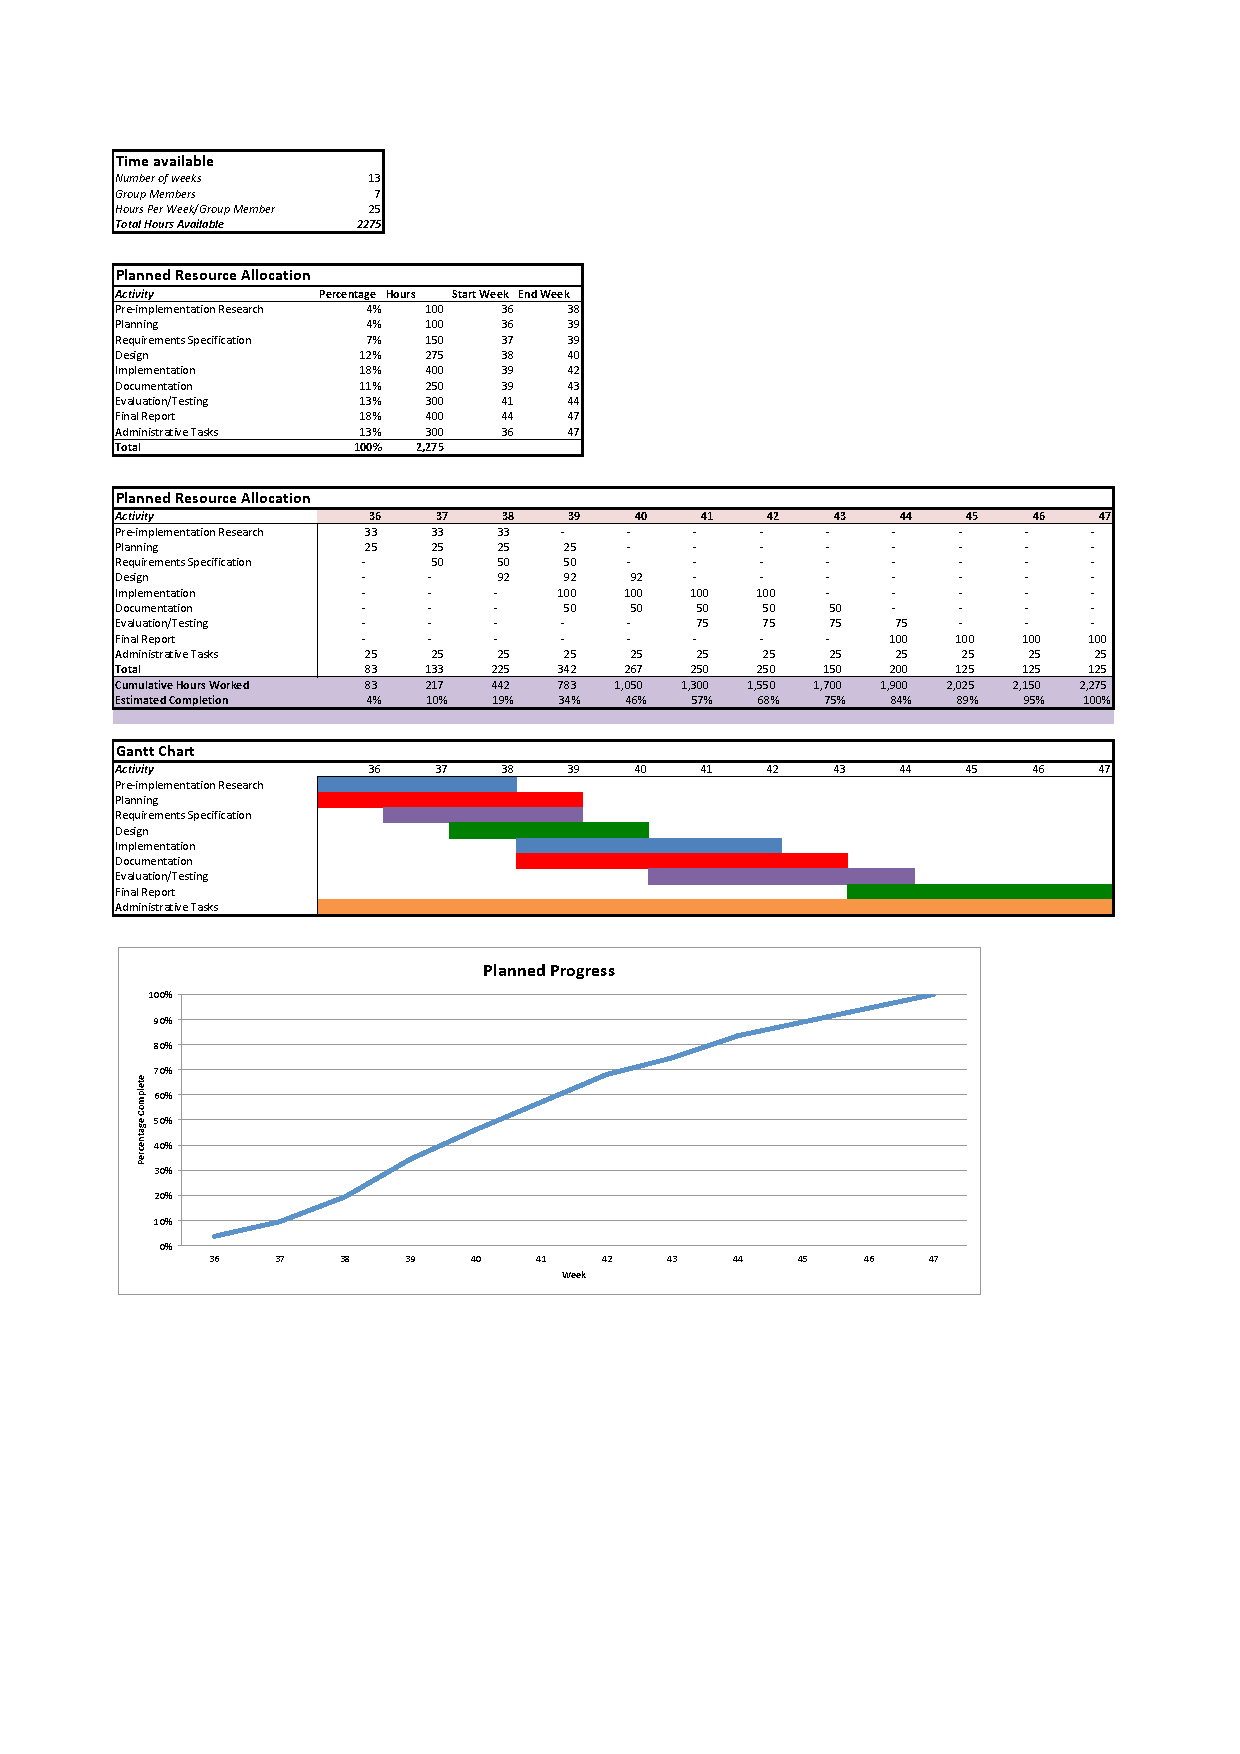
\includepdf{PlanReport/DetailedPlan}


\part{Design and Implementation Phase}\label{p2}
\setcounter{section}{0}
\addtocounter{chapter}{1}
% Activate the following line by filling in the right side. If for example the name of the root file is Main.tex, write
% "...root = Main.tex" if the chapter file is in the same directory, and "...root = ../Main.tex" if the chapter is in a subdirectory.
 
%!TEX root =  

\chapter{Requirements Specification}\label{reqspec}

\minitoc

\section{Purpose}
This requirements specification has been prepared for and accepted by SINTEF ICT (the customer) stating the requirements for the software system to be developed for the course TDT4290: Customer Driven Project. The requirements span two categories; functional requirements, describing the functionality the software needs to supply, and non-functional requirements, describing the development process.

The requirement specification, once accepted by the customer, will serve as a contract between the parties involved, being a guideline for design and implementation and the standard against which the product is evaluated.
\section{Introduction}
\subsection{Background and Similar Software}
SINTEF ICT is currently investigating new approaches to privacy protection of end-users. T�ndel and Nyre (2011) proposes a specific agent design for a machine learning approach to advice users on privacy actions based on:

\begin{itemize}
\item Past behavior using case based reasoning (CBR)
\item Similar users� behavior in similar situations using collaborative filtering (CF)
\end{itemize}

While there are systems for aiding users in making privacy related decisions, the majority of these systems rely in a large extent on the user pre-specifying his preferences and being prompted with messages about where the policy of a given site conflicts with the user�s preferences. Our design aims at being �low profile� or �non invasive�, that is able to make sensible decisions with as little interference as possible, and at the same time, given as little feedback as possible, able to cater for the dynamic nature of both web sites� privacy policies and user preferences with respect to privacy.

\subsection{Scope}

The primary aim of this project is the implementation of the core classification system described in T�ndel and Nyre (2011) to allow for testing the applicability of the suggested approach to predicting privacy preferences. Since the software is intended to be a part of a research project, a design that allows for testing of various hypotheses and models is required. This implies a highly modular design where the various components of the core system can be replaced. 

Furthermore, given the research nature of the project, less emphasis is placed on developing a complete stand-alone application. The core focus for our project will be on developing the underlying system and an interface for testing and parameter estimation. Hence two distinct systems are to be developed, both built around the same core functionality (I.E. the privacy advisor agent). Owing to the fact that this software is developed around a research project, the emphasis is on the first system:

\begin{enumerate}
\item A testing system that can be fed a knowledge base consisting of input-output mappings (P3p + context -> decision), and run interactive tests on a sample where the user is allowed to give feedback to the system and see the explanation for the recommendation. We envision a dual CLI/GUI (command line interface and graphical user interface) solution for this. In a final product, this testing system can also be used for the purpose of calibrating the model.
\item An end-user system that can run as a browser plug-in giving real time advice to the user as he browses the web.
\end{enumerate}

\subsection{Overview}
This document is organized as follows:
�	Section 2 gives an overview over the system; its requirements and user characteristics.
�	Section 3 presents four different use-case scenarios.
�	Section 4 presents specific functional and non-functional requirements.
\section{Overall Description}

\subsection{System Description}
The overall structure of the system is detailed in T�ndel and Nyre, and consists of the local CBR reasoning system, the remote/community collaborative filtering, both with their respective databases for storing information. This is in turn linked to an interface that is able to read and parse P3P policy files that are retrieved either from a local file (for the testing system) or by retrieving from the web.

 
Figure 1: End User System Flowchart

\subsection{User Interface}
Because of the research nature of the project, the customer considers the user interface to be of small importance. As the underlying algorithm/methodology is in an early development phase, the core focus is placed on producing a system for model testing and evaluation rather than an end user interface. 

\subsection{Hardware and Software Interface}
Being written in Java, the software requires a local copy of the Java Runtime Environment (JRE) installed on the computer. 

For the community functionality (collaborative filtering), a dedicated server running the filtering engine must also be available. Since this is basically a modified version of the local server, it has similar requirements, but as it presumably will hold a larger knowledge base, its hardware requirements will be greater, as both lookup time (computational demands) and storage demands will increase with the number of users. It may also require additional server/database software such as mySQL, CouchDB etc. 

\subsection{User Characteristic}

For this project we distinguish between two groups constituting the users of the product. 
\subsubsection{Developers/Researchers}
Firstly, developers/researchers that will be working on the testing and calibration of the underlying model and extending it to other policy types beside P3P etc. These users are the primary focus of our work. A research/developer is an expert user, and needs to be familiar with how privacy policies are coded in machine-readable form such as P3P, but also the software source codes in order to modify, extend and optimize the algorithms. 

\subsubsection{End Users}
Secondly, the end user who will be using the software in the form of a browser plugin that provides advice with respect to the users behavior on the Internet. A key objective for the project is that the agent is to be able to make good decisions and require as little feedback as possible from the user. To the extent interaction is needed, it should be able to clearly state an explanation for its decisions and allow the user to override in a simple manner.


\section{Use Cases}

The first use case illustrates a research setting where calibration/testing interface allows the user to load in a dataset of P3P policies and test the performance of the underlying model. The last three use cases illustrate the potential application of the system as a browser plugin that runs in the background monitoring the users activities and the web sites he is visiting. As previously stressed, the success of testing according to the first use case determines the extent to which the system described in cases 2-4 is implemented.

\subsection*{Case 1: Research/calibration}
In this case a researcher wants to test the properties of the underlying model. Using the Calibration GUI, he imports 50 P3P policies that are parsed. Further he designates that 40 of these are to be stored immediately in the knowledge base along with a corresponding action for each policy. 
The user now specifies the distance metric he wants to apply to each of the different components. Finally, he can either set the (importance) weights assigned to each of the policy components, or he can load the weights from a flat text file. Now that the configuration is complete, the ten policies withheld earlier from the sample can be classified. For each of the ten policies, the user can choose either to accept, or reject, and provide a reason for his rejection before proceeding to the next policy. 

\subsection*{Case 2: End user � local query, recommendation accepted, site rejected}
A user visits a previously unvisited website. The privacy agent tries to retrieve machine-readable privacy information from the site. When the policy is obtained it is parsed and a context object, consisting of the policy, domain, time of visit, and other contextual information, is created. The context object is compared to the local database for similar contexts. Since the user has visited sites with a similar policy previously, the comparison succeeds and the site is blocked based on data from the local database. The user agrees with this decision and navigates away from the site.

\subsection*{Case 3: End user � local query, site approved by recommender, recommendation accepted}
A user visits a previously unvisited website. As before, the system the system fetches the necessary data to do a local query. This query indicates, with sufficient confidence, that the site�s policy is acceptable. The user is then allowed to continue browsing with no intervention from the Privacy Agent.

\subsection*{Case 4: End user � global query, recommendation overridden}
As before, but in this case, no sufficiently similar cases are found locally. In this case the system will query the global server for similar users that have visited the same site to base its decision on this. In this case, site is blocked, but the user disagrees. He selects an override feature and gives a reason for why he overrides.

\section{Specific Requirements}

\subsection{Product perspective}
As described in Section 1.2, as the main goal of the project is to develop a testing framework for the core reasoning system. The secondary goal is to implement a user interface that can work as a stand-alone application to allow for actual user testing.

\subsection{Functional Requirements}
\begin{itemize}

\item The system should be able to parse a P3P file to instantiate the data as a privacy case/event/instance.
\item Based on past history (knowledge base), it should retrieve the cases most similar to the one presented.
\item Given the degree of similarity to past cases and the uniformity of action taken in the past, the system can either 
\begin{itemize}
\item Give the user a recommendation a recommendation or 
\item Pass the recommendation decision on to the community/CF system.
\end{itemize}
\item If passed on to the CF, the system will query a server for the most similar users and use the data on their decisions in similar cases to make a recommendation (along with local/CBR recommendation) 
\item Update the database with the recommendation.
\item Allow the user to view the explanation for the recommendation
\item Allow the user to overrule a recommendation. 
\item When overruling a recommendation, the user must be allowed to explain why the decision is made, e.g. one time occurrence, permanent rule, etc.	
\item Allow the user, if making a new general rule, to backtrack and alter previous cases
\end{itemize}

\subsection{Non-Functional Requirements}
\begin{itemize}
\item Implementation
\begin{itemize}
\item Code is written in Java following Sun Microsystems� conventions (http://www.oracle.com/technetwork/java/codeconvtoc-136057.html).
\item Third party libraries are to be documented with version numbers and to be included in the installation package.
\end{itemize}

\item Maintainability:
\begin{itemize}
\item Code repositories and version control: github is used as code repository and for version control.
\item User documentation is to be produced.
\item A well documented API is to be designed	
\item English (US) is to be used as language for naming convention for source code and filenames, and in code comments and documentation.
\item The code is to be designed in a modular fashion.
\end{itemize}

\item Performance: 
\begin{itemize}
\item For the final end-user product that will run as a browser plug-in, performance will be important, as the program should not be seen as a nuisance in getting work done.
\end{itemize}

\item Portability: 
\begin{itemize}
\item The testing/design system should be portable to any system with a JRE.
\end{itemize}

\item User interface:
\begin{itemize}
\item Two UIs are to be implemented: A command line interface (CLI) as well as a GUI is to be designed using Java/swing.
\item These interfaces are meant to facilitate testing the model framework.
\end{itemize}

\end{itemize}


\setcounter{section}{0}
\addtocounter{chapter}{1}
% Activate the following line by filling in the right side. If for example the name of the root file is Main.tex, write
% "...root = Main.tex" if the chapter file is in the same directory, and "...root = ../Main.tex" if the chapter is in a subdirectory.
 
%!TEX root =  

\chapter{Design}
\label{design}

\minitoc

\section{Purpose}
This document describes the design phase of the program, where the program architecture is established. Several critical decisions are made in this phase and the design and architecture decisions impacts the way the implementation phase proceeds as it defines how the final software system is decomposed into modules, and how these modules behave and interact with each other. Details regarding programming languages, algorithms, data structures, coding standards and other software engineering features must also be established prior to proceeding from this phase.

\section{Development Tools and Technologies} 
This section details some of the choices that were made regarding development tools and technologies for this project.

\subsection{Documents and Source Code Repositories}
For software projects of a certain scale, version control is an important technology that allows project members to work simultaneously against the same files without causing inconsistencies. Version control systems also allow for comparison with older versions, tracking changes and restoring previous copies in the case of errors.

For source code repositories and version control, \textbf{Git} was selected. Git is a distributed, open source version control system that is available for all platforms. Git is also used for hosting the \LaTeX documents that comprise this report. For other documents such as meeting minutes, agendas, status reports, time reporting and certain planning documents, Google Docs is used.


\subsection{Programming Languages}
\textbf{Java} is chosen as the primary programming language for implementing the majority of the code. Java is an object oriented programming language providing a level of abstraction appropriate for the task at hand in addition to a rich set of libraries, including the SWING library for GUI programming, and several libraries for networking. It also simplifies writing a browser plugin as major browsers such as Google Chrome and Firefox employ Javascript as 

\subsection{Databases}
For testing purposes, it has been decided on using flat file storage of privacy policy data using Java's \texttt{Serializable} interface. However, the output functionality is to be written in a generic fashion to simplify use of database systems such as MySQL, CouchDB and so forth. 

\subsection{Third Party Libraries}
 
For developing the CBR as well as P3P parsing components of the Privacy Advisor, a decision had to be made regarding the usage of third party libraries, either for components or for the entire CBR system. We basically considered two options with respect to the CBR system, the first was to use a full third party CBR system (jColibri) and the second was to use a third party system for the retrieval component of the CBR system (i.e. a k Nearest Neighbors (kNN) implementation).

\subsubsection{Third Party CBR System}
The customer (SINTEF ICT) suggested looking into an open source CBR library developed at the Universidad Complutense de Madrid.
 
jColibri is a CBR system that has been under development for well over 10 years and is a very comprehensive system allowing for database interfaces and several other features,  and is according to the customer, a popular choice in academia for CBR projects. It is also written in Java, which of course makes interfacing it simple from our own Java project.
 
However, its comprehensiveness also means that it takes more reading to understand and properly apply to the project at hand, and due to its size and poor documentation, jColibri was ultimately deemed unfit for the Privacy Advisor project. Due to the limited time resources available to this project, the risks associated with spending a large amount of time on a third party library that eventually would not be running was to high.
 
\subsubsection{Third Party k Nearest Neighbors Implementations}
Since kNN is a standard classification algorithm, there are several open source implementations available. Limiting the search space to Java implementations, a library called �The Java Machine Learning Library� (JavaML) was the primary candidate, as it provided a clean and simple interface and allowed for extracting confidence measures.
 
The problem with this library relates to the nature of distance metrics used in classifying privacy policies which is compositional in a way that is non-trivial to handle in JavaML. Furthermore, JavaML seems to operate only on arrays of floating point numbers, which means the distance metric must be defined in two stages; first mapping from �policy domain� to real numbers, then in terms of a metric on real vectors.

\subsubsection{P3P/XML Parser}
Looking for XML parsers on the Java platform, we found out that there are two different types of XML parsers we could use, the first being a DOM Parsers and the second one being a sequential access parser. The difference being that DOM parsers operate on the document as a whole, while sequential access parsers operates on each piece of the XML document sequentually.

We ended up using SAXParser, an internal sequential access parsers in Java. The task from here was to implement it, making the policy as an object with the fields of our choosing. It works by sequentially going through all elements of the XML document, and with easy string comparison, checking if the element is of the wanted ones.

\section{Standards}
To achieve clean and reusable code, the project has adopted Oracle's Coding Conventions for the Java Programming Language\footnote{http://www.oracle.com/technetwork/java/codeconvtoc-136057.html}. This is mentioned in the requirements specification due to the high likelihood of the customer having to change the source code for later adaptations.


\section{Architecture}
To implement the Privacy Agent, a class structure is built around the CBR agent model discussed in T�ndel and Nyre with certain additions and refinements to handle data structures, algorithms, IO and so forth. 

\setcounter{section}{0}
\addtocounter{chapter}{1}
% Activate the following line by filling in the right side. If for example the name of the root file is Main.tex, write
% "...root = Main.tex" if the chapter file is in the same directory, and "...root = ../Main.tex" if the chapter is in a subdirectory.
 
%!TEX root =  
% Activate the following line by filling in the right side. If for example the name of the root file is Main.tex, write
% "...root = Main.tex" if the chapter file is in the same directory, and "...root = ../Main.tex" if the chapter is in a subdirectory.
 
%!TEX root =  

\chapter{Implementation}\label{impl}

\minitoc

\subsection*{Purpose}
This chapter explains the implementation phase of the project it provides a more detailed description of particular key
details that were not decided on in the design phase. This relates in particular to choices regarding the particular CBR algorithms
(k-Nearest Neighbors) and the similarity measures describing how "equal'' two cases are. It also details the data structures that
are used to represent policies and how comparisons are done on these data structures.

\section{Algorithms}

\subsection{K-Nearest Neighbors}\label{kNN}

\emph{K-Nearest Neighbors} (k-NN) is a \emph{lazy, non-parametric} algorithm for classifying objects based on the classification of the nearest examples in a given feature space. k-NN is one of the simplest machine learning algorithms as it decides the classification based on a majority vote of, that is, an object is classified according to the most common classification of its $k$ nearest neighbors. The most critical component for the success of the k-NN algorithms is the definition of distance. This is discussed in Section~\ref{SimilarityMeasures}. 

For testing purposes, we have implemented a very simple kNN that sorts the example set (knowledge base) by distance from the object to be classified and returns the k nearest objects. This is obviously not an optimal approach being $O(n lg(n))$ where $n$ denotes the size of the knowledge base. This is not problematic for a small scale application such as ours where the knowledge contains less than 200 objects. If the system is to be scaled up, it would require a new kNN implementation, of which there are several available.


\subsubsection{Learning algorithms}\label{learnAlgos}
The learning algorithm updates the weighs that each property field is assigned in computing distances. The learning algorithm goes through the policies in the database and computes updated weights. The implemented learning algorithm is a simple one that for each weight goes through every policy and checks if it have been accepted or not. Then it returns the number of accepts divided by the number of policies for each weight.

By updating the weights like this we make sure that the system to some degree learns what the user wants. Thus, hopefully the system would be able to make a different conclusion next time if the user didn't agree on the conclusion the system came up with this time.

\subsection{Confidence Measure}\label{confidenceMeasure}
%% maybe to be put in design

\subsection{Distance Measures}\label{SimilarityMeasures}

\subsubsection{Definition}

Mathematically, a \emph{metric} or \emph{distance function} is a function that defines the \emph{distance} between two objects in a set. That is, it defines a notion of how far apart two objects are. In a purely mathematical sense, a distance function defined over a set $X$, $X\times X\longrightarrow \mathbb{R}$ that is required to obey the conditions of non-negativity, symmetry, sub-additivity (the triangle inequality) and identity of indiscernibles. 

Some examples of commonly used metrics are the Eucldean, Mahalanobis, and the Manhattan distance measures. These along with a few others are defined in the next section. These metrics have all in common that $\mathbb{R}^n\times \mathbb{R}^n\longrightarrow \mathbb{R}$, which in the case of comparing privacy policies and corresponding context information, is problematic as these, in their raw form contain large amounts of textual data. Two remedies could be proposed for this situation:

\begin{enumerate}
\item Provide a function to map privacy objects (P3P policies and context info) to real vectors.
\item Define a new metric that operates directly on privacy objects.
\end{enumerate}
 
%% NBNBNBNB!!!!
%% Formulae must be inserted!!
%%

\subsubsection{Common Metrics}

\begin{itemize}
\item \emph{Manhattan distance} is function computes the distance that would be travelled to get from one data point to the other if a grid-like path is followed. 
\item \emph{Hamming distance} is defined as number of positions in which a source and target vector disagrees.
\item \emph{Levenshtein distance} is based on Hamming distance but adds also operands as insertion, deletion and substitution. 
\item \emph{Ontology distances} are more based on compute semantic similarity of objects rather than their textual representation. For example distance between apple and orange is less then between apple and house. To calculate this distance you need some sort of logical tool like ontological tree. Where every leaf has a logical ancestor for example ancestor for apple will be fruit.
\end{itemize}
\subsubsection{Customer Advise}

In the paper "Towards a Similarity Metric for Comparing Machine Readable Privacy Policies", some of the problems of defining a similarity metric for privacy policies is discussed. A key topic is how the calculation of similarity between online 3P3 policies can be subdivided in two parts, \emph{local similarity} and \emph{global similarity}. This way, known metrics such as Levenshtein distance  can be applied to local distance. And for global similarity we can calculate a simple or weighted average of local distances, where the second one allows for amplifying the importance of particular attributes.

Another important topic is how system designers can apply domain knowledge to improve distance calculation. For example, for the recipient field identifying who data is shared with, there are certain values revealing that significantly more private information is exposed than others. Having private information retained by the website (recipient = "ours") is in a sense less critical than it being given away to third parties for commercial purposes (recipient = "other) or being public (recipient= "public"). So distance between unrelated or public is less than between ours and unrelated.

\subsection{Implementation}

\subsubsection{Bitmap Representation}
A bitmap (or bit string) is a way of representing a set of objects. It simply translates values from a set to a vector of fixed length, where each value has a specific place. For example over language $L=\{a,b,c,d\}$ for a sets $\{a,b,c\}$ a bit-map will look like $[1 1 1 0]$ where 1st integer represents $a$ and last integer represents value $d$. This way it doesn't matter what order the values are arranged and how many values are so set $\{d,b\}$ over same language $L$ will be $[0 1 0 1]$ where 1st value still representing value $a$, or more correctly said, absence of value $a$. Calculating intersections or unions over bitmaps $A$ and $B$ uses bitwise Boolean operators. Where union can be easily written as $(A_i \vee B_i)$ where i is the position in the vector, and the intersection $(A_i \wedge B_i)$.

Weighed bitmap is when each of the values is multiplied by its corresponding weight. Let us say on the language $L$ the weights are $a=1 b=2 c=4 d=3$, since bit-map over set $\{a,b,c\}$ is $[1 1 1 0]$ the weighed bit-map will be $[1*w_a 1*_b 1*_c 0*w_d]=[1 2 4 0]$. And for set $\{d,b\}$ it will be $[0 2 0 3]$.

\subsubsection{Privacy Policy Representation}

This section describes the data structures used to represent policies. On the top level, \texttt{policyObject}s contain P3P policy and context information (URL + time etc.). A P3P policy can have a varying number of \emph{statements}, some of them greatly differ from each other, and others are very similar. Each statement is build of four fields: data-collected, purpose, recipient and retention. Purpose, recipient and retention can contain one or many given values, the combination of what describe how the given data-collected may be used in the future. Data-collected is divided in four major fields: dynamic, user, third-party and business. Many different data-types can be collected in one statement.

For every data object that being described in a statement, we create a \texttt{Case}. A \texttt{Case} in a \texttt{policyObject} corresponds to a statement in P3P policy. It contains the purpose, recipient and retention, but a Case can only have one unique data type; this results that one statement can be translated to many cases. \texttt{policyObject} has a list of all its \texttt{Case}s and additional information that we find useful like time of the visit, location of the domain, and action decided upon by the CBR system or the user. Based on SINTEFs proposal the two levels of similarity, local and global are accounted for in implementation. 

\subsubsection{Bitmap Distance}

The distance function is to be a highly modular component of the CBR system. The default distance function implemented uses the bitmap data structure mentioned above, and is henceforth referred to as "Bitmap Distance". For the local similarity Bitmap Distance generates bitmaps for fields, retention, purpose, and recipient. This eliminates the problem that these fields can have a differing number of attributes.  Prior to computing the Hamming distance the bit-map is transformed into weighed bit-map by multiplying every attribute by its weight. Since data-type is a string value the bitmap representation would be impossible. The distance between data-types can be calculated by either string comparison or ontological tree. The Hamming distance for weighed bitmap is easy to implement it can be represented by Boolean expressions. With creation of bitmaps is a fast algorithm with a linear run-time. The easy way of predicting the result and fast run-time is the strengths of this implementation.



\subsubsection{Data-type-string similarity}
The way data type is structured in P3P policies makes it possible to calculate a data-type distance by just parsing data-type-string. Every data-type string has to start with one of the four previously mentioned fields, then after a dot a sub-field is followed after other dot a sub-sub-field. Let us say we have your simplified ontological tree just within the syntax of data-type-string with an "invisible" root node over those four fields. This way when we have two data-type-strings for comparison we can easily count number of ancestors from string A to string B. For instance String a is “user.home-info.postal” and B “user.bdate”. Number of nodes we need to take from stringA to stringB is 3. 

The weakness is that without weights it is more of string comparison than ontological tree.

It is possible to create a weight system so this algorithm will work like a full ontological tree. For example if each node had a value/weight it would be possible to simply take difference between StringA’s 1st 2nd and 3rd field and respectfully StringB’s fields.
 
Weights are the key to learning and adjusting this algorithm. They are greatly used in previously mentioned implementation of Hamming distance and can give great results in data-type analysis.

\subsubsection{ The global similarity }
The global similarity part was not as easy as creating a bitmap. The number of cases a policy can be is undefined, and the similarity of those cases can differ a great deal. Your solution was sum of minimal distance of each Case to a case in the other policy. For instance a caseA from policyA have distance 2, 3, 1 to cases in policyB that mean the distance caseA will have distance 1 to policyB. 

\begin{figure}[htpb]

\begin{verbatim}

Sum=0
For caseA in PolicyA
  Min=infinity
  For caseB in PolicyB
    Dist=Compare(caseA, caseB)
    If dist<min then
      Min=dist
  Sum=sum+min
Distance=sum
\end{verbatim}

  \caption{Algorithm for similarity computation.}
  \label{similAlgo}
\end{figure}
 

By choosing minimal distance between cases we guaranty that if two cases are identical the distance between them will be 0. But it also creates a problem, consider two policies policyA with {caseA1 caseA2 caseA3} and policyB with {caseB1 caseB2} where every case in A has minimal distance with caseB1. This way the properties of caseB2 will go unnoticed in the sum of distances between cases. We solved this problem by running algorithm twice but changing places of policy A and B the 2nd time and simply summing results.

The weakness of computing this way is that some of the distances will be counted twice, but user-privacy-safety wise is better to count some cases of minimal distance twice then leave a most distant case out.

There is some variations in this method. You can use maximum/minimum distance between cases or average of the sum. We choose minimum because this way we always try to find a best match between cases and policies. With an algorithm that will minimize error from computing twice, from a to b and b to a, minimum distance will give the best results. But in total picture if you use same algorithm that considers every case for every policy in your database the results will be proportional.




\section{Data Storage}


\subsection{Flat File Storage}



\subsection{Databases}

\section{User Interface}

\subsection{Model View Controller Architecture}
[Describe theoretically]

\subsection{Privacy Advisor Interface}
[Describe choices that have been made and reasons for differences from standard architecture]

\subsection{CLI}

\subsection{GUI}

\setcounter{section}{0}
\addtocounter{chapter}{1}
% Activate the following line by filling in the right side. If for example the name of the root file is Main.tex, write
% "...root = Main.tex" if the chapter file is in the same directory, and "...root = ../Main.tex" if the chapter is in a subdirectory.
 
%!TEX root =  

\chapter{Documentation}\label{doc}

\minitoc

This chapter provides documentation for the Privacy Advisor system. It gives an overview over the available source code documentation (JavaDoc), instructions for how to compile and install the system, and how it is used via. its GUI and command line interfaces.

\section{Source Code Documentation} 

The source code is documented using JavaDoc which is a tool that generates documentation in HTML format based on source code comments in Java, and is a standard part of the Java SDK. The JavaDoc for the Privacy Advisor system follows Sun Microsystems' style guide for writing JavaDoc comments\footnote{See: http://www.oracle.com/technetwork/java/javase/documentation/index-137868.html}. 

Source code documentation plays an important role in this project, as it is an early software prototype to be used in research which means that the code is then likely to be modified. The aim of the source code documentation is to supplement UML design documents to facilitate future development.



\section{Installation}


\subsection{Compilation in Eclipse} \label{LocalInst}
The simplest way to make the program run as a stand-alone program on a Java Virtual Machine is to compile the source code to a runnable jar file. This section covers how this is done in the Eclipse environment.

\subsubsection{Open Export Wizard}
This can be done by right clicking the project in Eclipse, choosing \texttt{Export}, type in \texttt{jar} in the new window that opens up and choose \textbf{Runnable Jar File}, before clicking \textbf{Next}. These steps are shown in the two figures \ref{exportFirstStep} and \ref{exportSecondStep}.

\begin{wrapfigure}{r}{0.4\textwidth}
  \vspace{-10pt}
  \begin{centering}
    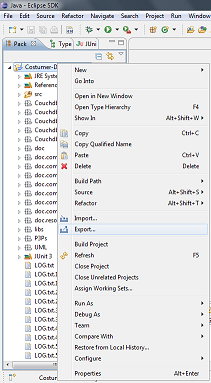
\includegraphics[width = .38\textwidth]{Documentation/export.png}
    \vspace{-10pt}
    \caption{First step: right click and choose "export".}
    \vspace{-10pt}
    \label{exportFirstStep}
    \end{centering}
  \end{wrapfigure}

  \subsubsection{Select GUI or CLI}
  The next step is to select which class file is to be the main class\footnote{Privacy Advisor has two files containing a main method. One is for running the CLI version, one for the GUI version.}; in the \textbf{Launch configuration} dropdown select either \texttt{PrivacyAdvisor} or \texttt{PrivacyAdvisorGUI}.

\texttt{PrivacyAdvisor} is selected to compile the command line version, and the \texttt{PrivacyAdvisorGUI} is selected for command line. Then choose the export destination, and choose \texttt{Package requires libraries into generated JAR} as the library handling. Pressing finish to start exporting the program. These steps are shown in figure \ref{exportLastStep}.


  \begin{wrapfigure}{l}{0.5\textwidth}
    \begin{centering}
      \vspace{-10pt}
      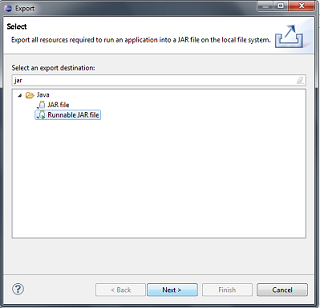
\includegraphics[width = .48\textwidth]{Documentation/export_jar.png}
      \vspace{-10pt}
      \caption{Second step: choose runnable jar.}
      \vspace{-10pt}
      \label{exportSecondStep}
    \end{centering}
  \end{wrapfigure}

\subsubsection{Configuration File}
Before running the program PrivacyAdviser.cfg has to be put in the same folder as the exported jar file. If the database file and the weights file at the same folder, their location have to be specified in the PrivacyAdviser.cfg file. 

\begin{wrapfigure}{l}{0.5\textwidth}
  \begin{centering}
    \vspace{-10pt}
    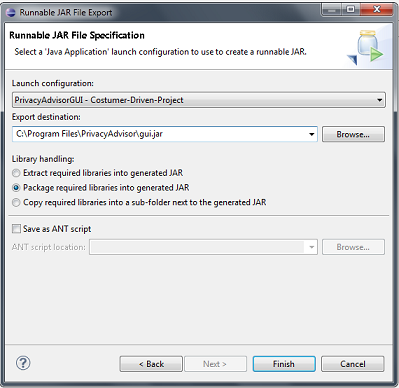
\includegraphics[width = .48\textwidth]{Documentation/export_last.png}
    \vspace{-10pt}
    \caption{Third step: choose launch config, destination and library handling.}
    \vspace{-10pt}
    \label{exportLastStep}
  \end{centering}
\end{wrapfigure}


\subsubsection{Sample Run}
To run the program, navigate to the folder where the jar file is stored and type the following command:

\framebox[1.1\width]{\texttt{java -jar filename.jar}}

Now the program should start (even if it's the cli or gui version). This is shown in figure \ref{runProgram}.

\begin{figure}
  \begin{centering}
    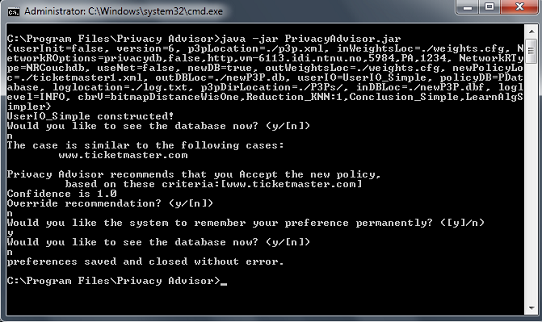
\includegraphics{Documentation/cli.png}
    \caption{Running the program.}
    \label{runProgram}
  \end{centering}
\end{figure}


\subsection{Server Installation}
The CouchDB server is a default Ubuntu installation on a VMware virtual machine provided by NTNU IDI, with CouchDB installed using the command:

\framebox[1.1\width]{\texttt{sudo apt-get install couchdb}}

The database server was configured via \emph{futon} (the default web interface, located at \texttt{localhost:5984\/\_util}) to provide a database entitled \texttt{privacydb}, with a non-administration user (details noted in default program configuration file).

\section{User Interfaces}
The Privacy Adviser consists, as mentioned in section \ref{LocalInst}, of two different user interfaces. The advantage of the GUI is that it's easier to see the contents in the database before and after the program runs. The command line interface better suited for repetitive tasks, in particular for batch type testing. The command line interface operates according to the options given when starting the program, either as command line parameters or through the configuration file. This is explained in detail in section \ref{cliExplained}.

\subsection{Command Line Interface} \label{cliExplained}
By running the program from the command line options can be set directly as command line parameters when starting the program. If no parameters are given, the options set in the PrivacyAdviser.cfg will be used. Options added as command line parameters have priority over configuration file options.

As an example consider the location of the database. By default, the options in PrivacyAdviser.cfg is set to replace the old database with the new database when the program exits. If the user wants to store the changes to a new database file, the \texttt{outDBLoc} parameter needs to be set to a new file.

There are two ways to change this. The first is to set the \texttt{outDBLoc} parameter at the command line. This will override the config file for this particular run. 

\framebox[1.1\width]{\texttt{java -jar privacyAdvisor.jar -outDBLoc newDatabase.db}}

More options can be added in this manner, and for the options that are not specified, the default options in the config file will be used. For a complete list of the options see table \ref{configTable}.

The second approach is to change the outDBLoc in the configuration file directly.

\subsection{Graphical User Interface}
When using the graphical user interface, the left hand pane gives an overview of the all the policies and cases in the database as a tree-structure. The right hand pane gives a similar view of how the new policy. This can be seen in figure \ref{guiFigure}. The GUI is started from the command line the same way the CLI is started.

\subsubsection{Obtaining Advice for a Policy}
When the GUI is stared, it automatically loads the database file, and displays the tree-structure. Pressing the \texttt{Run} button in the \texttt{Privacy Advisor} menu runs the CBR classifier and displays a message box containing an advice along with a measure of confidence and references to the sites on which the decision is based.

%%% TODO: edited hitherto

If we want to change the location of the database, the new policy or anything else we can press the \texttt{Configuration} button and make the changes in the \texttt{Configuration Editor} window that shows up. This Configuration Editor window is showed in figure\ref{guiConfig}.

 \begin{wrapfigure}{r}{0.5\textwidth}
     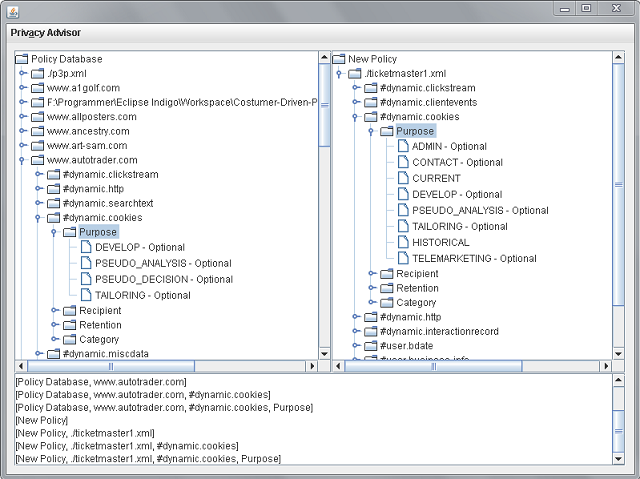
\includegraphics[width = .48\textwidth]{Documentation/gui.png}
     \caption{The GUI.}
   \label{guiFigure}
 \end{wrapfigure}

   \begin{wrapfigure}{r}{0.5\textwidth}
     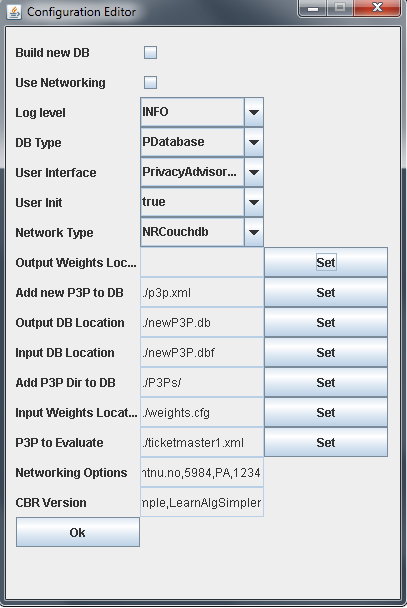
\includegraphics[width = .48\textwidth]{Documentation/gui_config.png}
     \caption{The GUI.}
   \label{guiFigure}
 \end{wrapfigure}


\subsubsection{Configuration Files}

Table~\ref{configTable} gives an overview over the configuration file parameters.

\begin{center}
  \begin{table}[h!]
    \label{configTable}
    \begin{tabular} { | l | l | p{7cm} | }
      \hline
      \textbf{Item} & \textbf{Datatype} & \textbf{Description} \\ \hline
      loglocation & string/filepath  & where the log is written to. can't be changed once the UI is  called. \\ \hline
      loglevel & string/logging level	& what level to log at. \\ \hline
      inDBLoc & string/filepath	& where to read the past history from. \\ \hline
      outDBLoc & string/filepath & where to write DB- defaults to where it reads from. \\ \hline
      inWeightsLoc& string/filepath & where to read the weights config file from. \\ \hline
      outWeightsLoc	& string/filepath & where to write DB- defaults to where it reads from. \\ \hline
      newDB & string/boolean & are we overwriting/ignoring an old database. \\ \hline
      p3pLocation & string/filepath & a p3p to be added to the history. \\ \hline
      p3pDirLocation	& string/FOLDERpath& a folder of p3ps to be added to the history. \\ \hline
      blanketAccept & string/boolean & accept the advisers recommendation. \\ \hline
      newPolicyLoc & string/filepath	& the new policy to be parsed. \\ \hline
      userInit & string/boolean	& true if some initialization occurs via the user interface. \\ \hline
      userResponse & string/action	& the response to the suggestion, if know beforehand. \\ \hline
      cbrV & string/CBR & parses for algorithms, etc to use. See CBR:parse(String). \\ \hline
      userIO & string/UIO	& the user interface to use. see Gio:selectUI. \\ \hline
      policyDB & string/policyDB & select the database type. see Gio:selectPDB . \\ \hline
      genConfig	& string/filepath & load an alternate configuration file. \\ \hline
      networkRType & string/classname & the name of a networkR class. \\ \hline
      networkROptions & string/commasepoptions	& the options necessary for the above networkR class. \\ \hline
      confidenceLevel & string/double & the confidence level at which the algorithm trusts itself; if below this, it uses the server's suggestion. \\ \hline
      useNet & string/boolean & whether to activate network functionality. \\ \hline
      \hline
    \end{tabular}
    \caption{Configuration file parameters.}
  \end{table}
\end{center}

\subsubsection{Building a Database}

\textbf{CLI}: To build a new database from a directory \texttt{P3PDir} holding P3P files, Privacy
Advisor can be called from the command line in the following fashion:

\framebox[1.1\width]{\texttt{PrivacyAdvisor -newDB  true -outDBLoc new.db
  -p3pDirLocation P3PDir}}

\textbf{GUI}: To build a new database in the similar fashion using the
graphical user interface, the configuration window can be set up
similarly to that illustrated in figure[XXXX].



\subsubsection{Loading and Viewing a Database}



\subsubsection{Parsing a P3P Policy}


\part{Evaluation and Summary}\label{p3}

\setcounter{section}{0}
\addtocounter{chapter}{1}
% Activate the following line by filling in the right side. If for example the name of the root file is Main.tex, write
% "...root = Main.tex" if the chapter file is in the same directory, and "...root = ../Main.tex" if the chapter is in a subdirectory.
 
%!TEX root =  

\chapter{Project Evaluation}\label{eval}

\minitoc


The final phase of the project consists of evaluating the actual outcome of
the project work and the processes that have led to the outcome. It
seeks to answer questions such as:

\begin{itemize}
\item Has the project acheived its major objectives?
\item In what areas could a better result have been achieved?
\item What could be done differently to acheive a better result?
\item How well did planned resource use reflect actual resource use?
\end{itemize}

The first section evaluates the software system in terms of the
objectives and requirements worked out prior to design and
implementation.  Sections \ref{toolseval} and \ref{resourceUse}
evaluate the appropriateness of the tools used in developing the
system and the resources committed to the project in manhours relating
to the original project plan. Finally, section \ref{courseEval}
evaluates the course as a whole.

\section{Software Evaluation}

This section contains the project team's evaluation of the software
system that has been produced.

\subsection{Key Objectives}

As discussed in Section~\ref{mandateObjectives}, the main objectives of the project were:

\begin{enumerate}
\item\label{itemTestFW} Implementing a testing framework of CBR based privacy agent that is able to make privacy decisions based on previous user behavior.
\item\label{itemCollaborative} Implement the community system/collaborative filtering part of the agent.
\item\label{itemExtend} Extend the system to other standards for machine readable privacy policies.
\item\label{itemBrowser}Implement the system as a browser plugin. 
\end{enumerate}

Objective~\ref{itemTestFW} were considered the clearly most important for the project, being a prerequisite for the remaining objectives. The fuctional requirements section (Section~\ref{funcRequirements}) in requirements specification goes further in detail on what the first objective entails.

\subsection{Evaluation}
The project team realized quickly that there were insufficent resources to meet Objectives 3-4, so focus was shifted to the first objective while, there was planned for working towards the second objective at the end of the project period. With respect to the first objective, the \emph{current Privacy Advisor system provides all the features listed in the requirements specification}. The second objective is partially realized. The core Privacy Advisor system has functionality extending the CBR for networking, and work on a collaborative filtering system has been started on a server machine at NTNU. The features supported by this system is however limited.


%%TODO: refer to testing results

\section{Tools}\label{toolseval}

Referring to choices discussed in section~\ref{DevTools}, the key
software tools and languages used are Java, Git, and Google
Docs. 

\subsection{Programming and Implementation}

\subsubsection{Java}
The choice of programming language for the project was very much up to the
project team as the customer had no particular preference, and the
project did not require anything beyond what is catered for by most
general purpose languages. \textbf{Java} was therefore selected 
selected as implementation language based on the following points:

\begin{itemize}
\item All team members had some previous experience in Java
  programming from previous coursework.
\item Good documentation and a large amount of third party libraries
  available on the web.
\end{itemize}

While all team members did have a Java programming background, there
were clearly vast differences in skill levels. This was the cause of
some frustration and extra work. In retrospect, more time should have been spent
on clarifying background and interests of each team member so as to
better allocate workload. Some will also argue that a more
"light-weight'' programming language, such as Python, would have been a
better choice, even despite the lack of previous experience.

\subsubsection{Git/GitHub}
Git and GitHub were chosen as version control system (VCS) and code
repository. Several team members had only marginal experience with
VCSs and did not commit to learning this in a serious manner, which
led to somewhat slow progress in the start. However, once these problems
were resolved, it can be agreed that Git has served its purpose well.


\subsection{Reporting and Organizational Tools}
Google Docs was used as repository for all "temporary'' documents such
as agendas, status reports, drafts and so forth. All "major''
documents were typeset in \LaTeX and stored at the GitHub repository.

\subsubsection{Google Docs}
There were no significant issues with Google Docs. It provided a good
framework for sharing binary files such as spreadsheets, presentations and so forth which
are not catered well for by most version control systems.


\subsubsection{\LaTeX}
Being the de-facto typesetting system for academic writing, and the
only one that some group members had experience with, \LaTeX was
chosen for writing the final report as well as all phase documents. As
with GitHub, though to a lesser extent,  there was a lack of commitment to learning by certain
group members, causing frustration and extra work on a later stage
in the project.


\section{Resource Use}\label{resourceUse}

Figures~\ref{perActivity} and \ref{actualPlannedCuml} illustrate
the discrepancies between actual and planned time use on all
activities, both cumulative over time and over each phase of the
project. It is updated as by the end of the last week of the project.

\begin{centering}
  \begin{figure}[h!]
    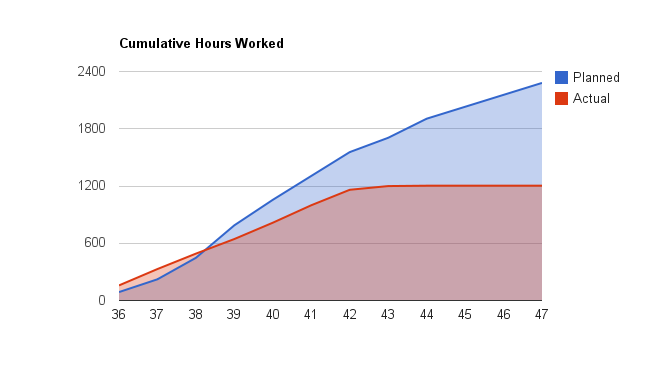
\includegraphics[width = \textwidth]{Evaluation/actual_v_planned_cuml}
    \caption{Actual vs. planned time. Cumulative over project span.}
    \label{actualPlannedCuml}
  \end{figure}
\end{centering}

As shown in Figures~\ref{perActivity} and ref{perActivityPct}, there are a few important discrepancies between the project plan and how the project indeed turned out. Firstly, there was a shortage of approximately 300 hours. This was quite evenly spread among most team members, with the exception of the team members with administrative responsibilities who had a significantly higher workload. The uneven workload also reflects an uneven background in academic writing which meant a large portion of the workload with this report was taken on by a few select team members.

Secondly, while the percentage workload between activities was quite well anticipated, there were some noticeable exceptions. One key pattern to notice is that while the design and implementation related activities required less time than initially planned, administrative work and planning required more work than planned. The overrun is most obvious for the administrative tasks part. One important lesson to take away from this is that a project team of a given size does need a major amount of administrative work. Another important reason for this overrun was initial problems with setting up the code repositories.

\begin{centering}
  \begin{figure}[h!]
    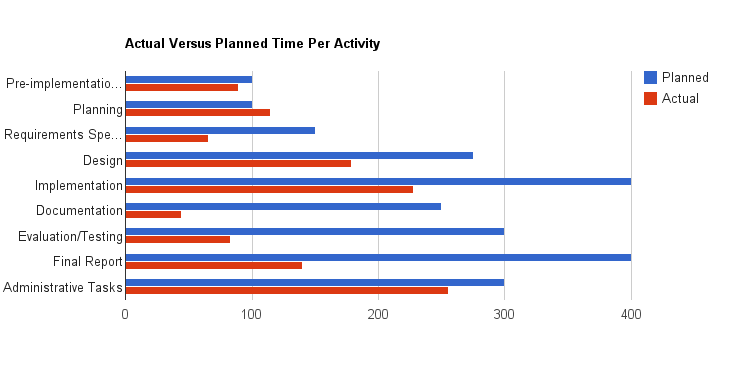
\includegraphics[width=\textwidth]{Evaluation/time_per_activity}}
    \caption{Actual vs. planned time. By project phase, in hours.}
    \label{perActivity}
  \end{figure}
\end{centering}

With respect to the relatively fewer hours spent on designing and implementing the system, a portion of this can be explained by the fact that a major portion of the design was clear from the beginning given that the system was to be based on the CBR framework. This and the fact that Java was decided on early on as programming language, severely limited the possible designs available. The implementation phase also required fewer hours than expected. This was in part due to the fact that the team did not realize all the objectives that were set (networking is only partially complete), and that work was divided well among team members. Interfaces were also built quite early on in the project so that adding on modules to existing code proved simple.


\begin{centering}
  \begin{figure}[h!]
    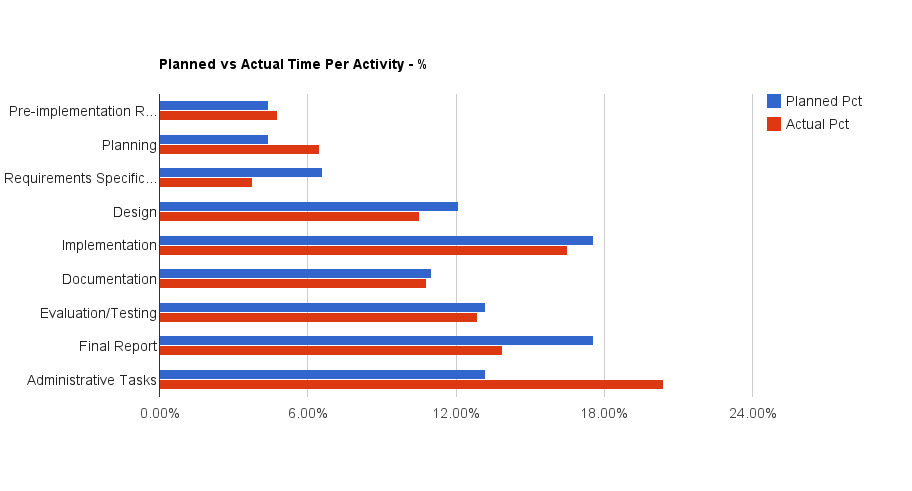
\includegraphics[width=\textwidth]{Evaluation/time_per_activity_pct}
    \caption{Actual vs. planned time. By project phase, in percentage of total time.}
    \label{perActivityCUml}
  \end{figure}
\end{centering}

\section{Risks that Occurred}

Referring to the discussion in section~\ref{riskReport}, we can state
in retrospect that few of the risks we anticipated occurred, at least
with major consequences. Some problems occurred building a P3P
parser (risk item 3), causing some initial delays as it took longer time than
anticipated to get the system fully working. This problem was in part
due to some unclear notions in the specification of the dataobjects
storing P3P objects.

Furthermore, the project has not proceded without any conflicts. While
roles and responsibilities were agreed on early on in the project
phase, it turned out that these initial assignments did not distribute the
workload very evenly. 


\setcounter{section}{0}
\addtocounter{chapter}{1}
% Activate the following line by filling in the right side. If for example the name of the root file is Main.tex, write
% "...root = Main.tex" if the chapter file is in the same directory, and "...root = ../Main.tex" if the chapter is in a subdirectory.
 
%!TEX root =  

\chapter{Conclusion}\label{conclusion}

\minitoc

\section{Summary and Final Remarks}

This project has designed and implemented a privacy agent based on the
research ideas set forth by SINTEF. The Privacy Advisor software  is a
case based reasoning engine that can provide advice 
with regard to P3P privacy policies given knowledge of previous user
actions. Both the idea and the software remain work in progress,
which is reflected by the system's user interface which is oriented
towards testing. It is built in a modular fashion, so that the
knowledge base, the retrieval algorithm and the similarity metrics, which are likely to be the
parts of the system that require most of the tweaking, can
be substituted without affecting the remainder of the software.



\section{Future Development}

To conclude this report, we look at the some important challenges that
must be addressed in order to further the Privacy Advisor system to a
end-user product.

\subsection{Testing}
For the Privacy Advisor system to be truly valuable, it has to be made
available to end users; the most likely realization being in the
form of a web-browser plugin. For this to occur, much testing is still
required. This testing is a more involved type of testing than the standard
unit testing that the Privacy Advisor system has been through at present.

For the system to actually be successful it has to provide accurate predictions
of users' Internet decisions so that it can provide good privacy protection
without being invasive in the users' day-to-day Internet activities. This type
of testing will require putting together a group of test users and monitoring their
activities over a \emph{prolonged period of time}\footnote{The time aspect is stressed here
as the system will need time to actually learn the user's preferences.}. 

The project team feels that most important and time consuming part of future development lies
in this area. Designing appropriate measures and testing routines for evaluating the performance
of the CBR agent is probably the main obstacle on the way towards realizing the design.

\subsection{Collaborative Filtering} %% TODO: Nicholas: verify
One of the key improvements to the current Privacy Advisor system is the
collaborative filtering/community portion of the system. While the interface
for a networking system is well integrated in the CBR system, the current 
network resource has limited features. Furthermore, this component of the system
will also require a prolonged period of testing, as a substantial amount of data.

% issues with duplicate policies on server, current state, proposed
% fix, sintef solution and problems with storing per user basis

\subsection{Distance Metrics and Algorithms}
The success of the CBR system in prediciting user preferences relies
in a large extent on the system's ability to accurately model the way
users actually compares two policies. This means that the one of the
most critical components of the CBR system is the distance metric
class. While a designer may have some intuition of how users may
compare two policies based on his own preferences, what in the end
provides a good fit  is an empirical question that will be subject to
verification through a testing process as discussed above.

In Privacy Advisor, a learning algorithm has been used as an aid in
improving the distance metric. However, the learning algorithm itself
is also a matter of debate: how quickly should it adjust the weights
in the distance metric as a response to new information? Questions
related to this remain unanswered in this project, and will likely be
a starting point for future research.

\subsection{The Current State of Internet Privacy Policies}
Finally, some words about the current state of Internet privacy policies. While P3P represents
an effort towards a machine readable standard for privacy policies, it is far from being adopted
universally. At present several standards seem to coexist, so a finalized system would have to
be able to handle several different standards.

Also posing significant problems to the effectiveness of privacy enhancement software is fact 
that there are little in the way of legal regulations of privacy protection online\footnote{See for instance:
http://www.nytimes.com/2011/11/20/opinion/sunday/a-push-for-online-privacy.html?_r=1&ref=opinion.}.
At present, businesses are free to arbitrarily change their privacy policies without noticing users,
and very little effort has been made towards verification or enforcement of policies. This means that currently,
the privacy policies cannot be the only input to a \emph{truly} trustworthy privacy enhancement software.




% Appendices
\part{Appendices}
\appendix
\Alph{chapter}
\setcounter{chapter}{1}
\documentclass[12pt, fullpage, oneside]{report}

\begin{document}

\title{Test Plan}

\subsection*{Test plan}
This is the test plan for the "Privacy Advisor" application requested by SINTEF ICT. This test plan is based on IEEE829-1998, the IEEE standard for software test documentation, with some adaptions to fit this project better. The purpose of testing is find bugs and errors and correct them, and to make sure the program is working as expected. The purpose of this test plan is to make sure the tests will be executed as planned, and that they are well documented.

\setcounter{tocdepth}{1}

\section{Test Methods}
There are two main types of software testing: black-box testing and white-box testing.
		
\subsection{Black-box testing}
This is a method that test the functionality of an application. For this type of testing, knowledge about the application's code and structure is not required. The test cases are based on external descriptions of the software, e.g. specifications, functional requirements or designs. Black-box tests are usually functional, but they can also be non-functional. This type of testing can be applied to all levels of software testing.
		
\subsection{White-box testing}
This method is used for testing internal structures of an application. For white-box testing it is required to have both knowledge about the code and structure of the application, as well as knowledge about programming to design the test cases. This type of testing is normally 	done at unit level where it can test paths within a unit or paths between units, but it can also be used at integration and system levels of testing. This method can uncover many errors and problems, but it is not a good test method for finding out whether the program is fulfilling the requirements or not.

\section{Testing approach}
Our main focus will be on white-box testing. This is a program that is going to be used for research, which means that black-box testing will not be very useful as the client want to work on and test algorithms themselves. Our main task is to deliver a good framework with the necessary tools, and a working, learning algorithm so that further testing can be done with ease. Since one of the system requirements is high modularity, it will be a goal to have the tests be as little dependent on other modules as possible. There will be no training needs, as the testers are also involved in the programming.

		\subsection*{What will be tested:}
			\begin{itemize}
				\renewcommand{\labelitemi}{$\bullet$}
					\item \textbf{Unit testing:} This will be used for testing the functionality of the modules, so that we can ensure that they are working as intended.
					\item \textbf{Learning of our algorithm:} As our algorithm is based on case-based reasoning (CBR), it will be important to test that it is learning from new data.
			\end{itemize}

		\subsection*{What will \underline{not} be tested:}
			\begin{itemize}
				\renewcommand{\labelitemi}{$\bullet$}
					\item \textbf{Usability testing:} This program is intended for further research by the client, and not for use by customers. Since we are not delivering a program ready for users, there is no need to perform end-user tests to see how users interact with the 							program, and whether the product is accepted by users or not.
					\item \textbf{Interface testing:} For the same reasons we will not perform any tests on the quality of the GUIs. The GUIs that will be included is there to make testing easier for the client, not to provide the best possible interaction with end-users.
					\item \textbf{Run time:} We will not do designated tests for checking and optimizing the run time. This is because the main classification algorithm can be easily changed. Run time will only be looked into if the program is very slow even for small data sets.
			\end{itemize}
		
	\section{Test case overview}
		This is the test cases and their identifiers. The identifiers are named UNIT-XX, where XX is the number of the test case.
		\vspace{8 mm}
		
		\textbf{Unit tests:}
		\begin{itemize}
			\renewcommand{\labelitemi}{$\bullet$}
				\item UNIT-01: Command line interface (CLI) functionality
				\item UNIT-02: P3P parser
				\item UNIT-03: Local database
				\item UNIT-04: Graphical user interface (GUI) functionality
				\item UNIT-05: Algorithm classification
				\item UNIT-06: Algorithm learning
				\item UNIT-07: Packet passing through network to community database
		\end{itemize}

		\vspace{8 mm}
		This is the test case template for the unit tests.
		\vspace{8 mm}

		\begin{center}
			\begin{tabular}{ |  p{4cm} | p{10cm} | }
				\hline
				Item & Description \\ [3pt] \hline \hline
				Name & The name of the test \\  [3pt] \hline
				Test identifier & The identifier of the test \\  [3pt] \hline
				Person responsible & The person responsible for making sure the test is executed correctly and on time. \\  [3pt] \hline
				Feature(s) to be tested & What kind of functionality that is being tested. \\  [3pt] \hline
				Pre-conditions & What code and environment that has to be in place before the test can be executed. \\  [3pt] \hline
				Execution steps & Stepwise explanation of how to perform the test. \\  [3pt] \hline
				Expected result & The expected output/result for the test to be successful. \\  [3pt] \hline
			\end{tabular}
		\end{center}

	\section{Test cases}
		See the appendix for the test cases.

	\section{Test pass / fail criteria}
		A test is passed if the given execution steps and input produce the expected results. If they do not, the test is failed.

	\section {Test schedule}
		This is the table for when the UNIT tests are scheduled to start.

		\begin{center}
			\begin{tabular}{ |  p{5cm} | p{5cm} | }
				\hline
				Test identifier & Execution date \\ [3pt] \hline \hline
				UNIT-01 & October 22nd \\  [3pt] \hline
				UNIT-02 & October 24th \\  [3pt] \hline
				UNIT-03 & October 26th \\  [3pt] \hline
				UNIT-04 & October 29th \\  [3pt] \hline
				UNIT-05 & October 29th \\  [3pt] \hline
				UNIT-06 & October 29th \\  [3pt] \hline
				UNIT-07 & November 12th \\  [3pt] \hline
			\end{tabular}
		\end{center}

\section{Risks and contingencies}
For some of the tests we will not be able to test every possible input / output. So there is a chance a test will pass for all the combinations we will be testing for a specific test case, but still fail at some later point for some other combination. This can be a problem for the tests UNIT-02 P3P parser, and UNIT-05 Algorithm classification.

The P3P policies have a huge variety in which elements they contain, and certain elements have a N-to-1 relation, so it will be impossible to test if everything is parsed correctly for every possible P3P policy. The best way to prevent this is to handpick a set of policies that have as different content as possible, so that as many of the extremes as possible will be covered.

We got the same issue for testing the algorithm classification. There is simply too many combinations of learning base and input to cover everything. So again we have to do our best with regards to also covering as many extremes as possible.


\end{document}
% Activate the following line by filling in the right side. If for example the name of the root file is Main.tex, write
% "...root = Main.tex" if the chapter file is in the same directory, and "...root = ../Main.tex" if the chapter is in a subdirectory.
 
%!TEX root =  

\chapter{Templates}

\subsection{Status Reports}

\subsection{Meeting Notes}

\subsection{Testing}

\subsection{Time Reporting}

%\bibliographystyle{plain-annote}
%\bibliography{mybibliography}


\end{document}
\end

